% ---------------------------------------------------------------------------
% Section 6: The institutional comparison, read after the transient.
% ---------------------------------------------------------------------------

\section{The institutional comparison}
\label{sec:institutional}

Environment B (\S\ref{sec:env-b}) is a subgraph of the same population in which
every member sees every other and proposing costs $c_B$. It is compared with the
mediated market, Environment A, over a grid of ten subgraph sizes and four costs,
ten seeds per cell, against two versions of A: the oracle, and the learned ranker.
Welfare is averaged over rounds 250 to 299, after the transient, and B's welfare
is on the common basis that scores every agent B excludes at what A would give it
(Figure~\ref{fig:institutional}).

At the lowest cost, $c_B = 0.01$, B beats A over a range of sizes. With
Benjamini--Hochberg correction over the forty cells, \nBeatsOracle{} cells beat the
oracle A, at sizes $\beatsOracleMin$ to $\beatsOracleMax$, and \nBeatsNcf{} beat the
learned-ranker A, at sizes $\beatsNcfMin$ to $\beatsNcfMax$, all at $c_B = 0.01$.
The largest difference is at size $\bestOracleSize$ against the oracle,
$\bestOracle$ $[\bestOracleLo, \bestOracleHi]$, and at $\bestNcfSize$ against the
learned ranker, $\bestNcf$ $[\bestNcfLo, \bestNcfHi]$. At $c_B \ge 0.05$ no cell
beats A after correction, and B falls further behind as the cost and the subgraph
grow.
The margin over the learned ranker is the larger one because that A's own welfare
is lower, $\welfareANcf$ against $\welfareAOracle$, although its exposure has by
then converged to the oracle's (\S\ref{sec:transient}). Why its welfare is lower
was not tested; the reading offered in \S\ref{sec:transient}, the right agents in a
different order, is consistent with the numbers and unmeasured.

The same grid read over its first five rounds, on the same seeds (a check added
after the late-window result was read), finds no
cell in which B beats the oracle A: every cell's mean is negative, and A beats B
after correction in \nABeatsFive{} of the forty. At size 0.65 and $c_B = 0.01$ the
difference is $\fiveCell$ $[\fiveCellLo, \fiveCellHi]$ over rounds 0 to 4 and
$\bestOracle$ over rounds 250 to 299. A comparison read at five rounds and one read
after the transient therefore point in different directions, for a quantity that
involves no learning on A's side once the oracle's thresholds have settled. This
experiment shows the difference and does not isolate its cause. In a gate regime
that never binds ($\phi = 0.2$, read at five rounds, ten fresh seeds) size 0.65
ranks first of ten at $c_B = 0.01$, as registered, with a mean of
$\inertBest$ $[\inertBestLo, \inertBestHi]$, positive over the same five rounds in
which the shipped gate gives $\fiveCell$. The sign of the early comparison thus
depends on the gate as well as on the horizon, and the two were not varied
together in one grid.

\begin{figure}[t]
\centering
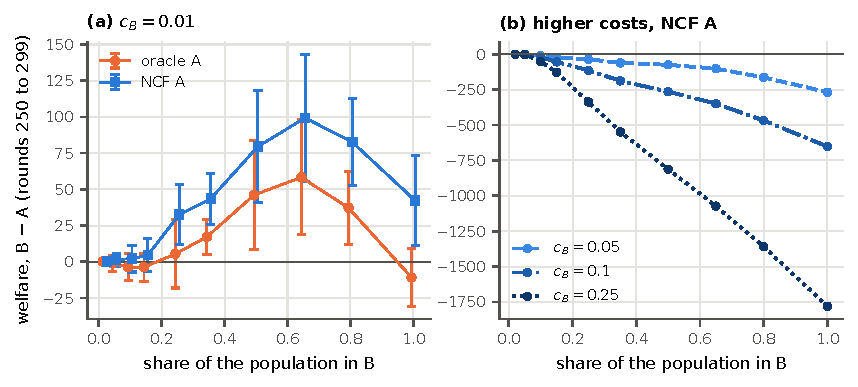
\includegraphics[width=\linewidth]{figures/institutional}
\caption{Welfare of Environment B minus Environment A over rounds 250 to 299, ten
seeds per cell, on the common basis. (a) $c_B = 0.01$ against the oracle A and the
learned-ranker A, mean with 95\% $t$ interval. (b) Higher costs, against the
learned-ranker A, mean. Source:
\texttt{data/processed/horizon/e15\_institutional/}.}
\label{fig:institutional}
\end{figure}
